\chapter{量子力学的形式体系}\label{ch:b3:quantum-formalism}

取三片偏振片。其中两片以 $90^\circ$ 交叉放置，
完全挡光；把第三片插入二者之间，使其成 $45^\circ$，
光便\emph{穿过}——增加一个障碍，反而打开了通路。
把偏振片看作筛子的图像经不起这个实验；
留下来的是线性代数：光子的偏振是一个
\emph{矢量}，每片偏振片沿某一轴对其测量并投影，
而概率即分量的模方。本章将这套代数确立为
量子力学真正的基础。前几章的波函数
只是一件具体的外衣，
包裹着更抽象的本体：态是\omterm{def:b3:quantum-formalism:state}{希尔伯特空间}中的矢量，
\omterm{def:b3:quantum-formalism:observable}{可观测量}是\omterm{def:b3:quantum-formalism:observable}{厄米算符}，测量值是\omterm{def:b3:quantum-formalism:observable}{本征值}，
概率是标量积的模方，演化由
\omterm{def:b3:hamiltonian-mechanics:hamiltonian}{哈密顿量}生成。五条基本假设，在我们已经计算过的一切中都已起作用，
——一经清楚表述，它们便足够强大，
足以处理直线上的波无法描述的系统：光子的
偏振、电子的自旋，以及中微子——其身份会
在穿越地球时发生振荡。

\section{态是矢量}

\begin{definition}[态空间、右矢与左矢]\label{def:b3:quantum-formalism:state}
\index{希尔伯特空间}\index{右矢}\index{左矢}
量子系统的态构成一个带内积的复矢量空间，
即\emph{希尔伯特空间} $\mathcal H$（其数学
在本科三年级数学分册中展开）。态
是一个矢量，记作\emph{右矢} $\ket\psi$，并归一化：
$\braket\psi\psi = 1$。两态的内积为复数
$\braket\varphi\psi$，对第一个变元共轭线性，
且 $\braket\varphi\psi = \braket\psi\varphi^*$。取标准正交
基 $\{\ket{e_i}\}$，
\[
\ket\psi = \sum_i c_i\ket{e_i} , \qquad
c_i = \braket{e_i}\psi , \qquad
\sum_i|c_i|^2 = 1 .
\]
前几章的波函数是
$\ket\psi$ 沿位置方向分量的族：$\psi(x) =
\braket{x}{\psi}$；并未丢失任何信息，而具有\emph{有限}
态空间——这在波的图像中不可想象——也变得可以描述。
\end{definition}

\begin{example}[光子的偏振：二维世界]\label{ex:b3:quantum-formalism:polarization}
沿 $z$ 轴传播的光子，其偏振态位于一个
\emph{二维}\omterm{def:b3:quantum-formalism:state}{希尔伯特空间}中，基为 $\ket H$（水平）
与 $\ket V$（竖直）。偏振角为
$\theta$ 的光为叠加态：
\[
\ket\theta = \cos\theta\,\ket H + \sin\theta\,\ket V ,
\]
圆偏振则为复组合 $(\ket H \pm
\iu\ket V)/\sqrt2$：系数为复数，并非
装饰，而是物理。一切量子两能级系统——自旋、氨
分子、超导量子比特——都属于同一矢量空间，
只是以不同的外衣出现。
\end{example}

\begin{omfigure}
\begin{tikzpicture}[font=\small, >=Stealth]
  \draw[->] (-0.3,0) -- (3.3,0) node[right] {$\ket H$};
  \draw[->] (0,-0.3) -- (0,3.3) node[above] {$\ket V$};
  \draw[->, omDef, very thick] (0,0) -- (35:2.9);
  \node[omDef, anchor=west] at (35:3.0) {$\ket\theta$};
  \draw[dashed, omThm] (35:2.9) -- ({2.9*cos(35)},0);
  \draw[dashed, omExo] (35:2.9) -- (0,{2.9*sin(35)});
  \node[omThm, anchor=north] at ({2.9*cos(35)},-0.08) {$\cos\theta$};
  \node[omExo, anchor=east] at (-0.08,{2.9*sin(35)}) {$\sin\theta$};
  \draw (1.0,0) arc (0:35:1.0);
  \node at (17:1.35) {$\theta$};
  \node[align=left, anchor=west] at (5.3,1.7)
    {沿 $\ket H$ 的概率：$\cos^2\theta$\\[2pt]
     沿 $\ket V$ 的概率：$\sin^2\theta$};
  \node[align=left, anchor=west, font=\footnotesize] at (5.3,0.45)
    {（本科一年级分册中的马吕斯定律，\\改读为玻恩定则）};
\end{tikzpicture}

{\small 偏振态作为矢量：其分量在
检偏器基下的平方即为各测量结果的概率——几何变为
概率。}
\end{omfigure}

\section{可观测量是算符}

\begin{definition}[可观测量]\label{def:b3:quantum-formalism:observable}
\index{可观测量}\index{厄米算符}\index{本征值}
一个\emph{可观测量}是线性算符 $\hat A$，作用于 $\mathcal H$，
且为\emph{厄米的}：$\braket{\varphi}{\hat A\psi} =
\braket{\hat A\varphi}{\psi}$，对所有态成立（用矩阵语言，
$A = A^{*\top}$）。其\emph{本征态}与\emph{本征值}，
$\hat A\ket{a} = a\ket{a}$，承载着全部物理：$a$ 即为
可能的测量值。常见例子：位置（$\hat x$：
乘以 $x$）、动量（$\hat p = -\iu\hbar\,\dd/\dd x$），
能量（$\hat H = \hat p^2/2m + V(\hat x)$）——以及二维中的
任一厄米 $2\times2$ 矩阵。
\end{definition}

\begin{theorem}[为何要求厄米]\label{thm:b3:quantum-formalism:hermitian}
\omterm{def:b3:quantum-formalism:observable}{厄米算符}的\omterm{def:b3:quantum-formalism:observable}{本征值}为实数，且\omterm{def:b3:quantum-formalism:observable}{本征值}不同的本征态
彼此正交；在本书涉及的空间中，其
本征态构成 $\mathcal H$ 的一组标准正交基（
\emph{谱定理}，有限维情形已在本科二年级
数学分册中证明；对无界算符 $\hat x$、$\hat p$，
$\hat H$ 的完整表述属于本科三年级谱理论，且
在本阶段不加证明地承认）。测量值必须为实数，且可区分的结果
必须彼此正交：厄米性恰好是使算符
能够表示测量的条件。
\end{theorem}

\begin{proof}[部分证明]
$a\braket aa = \braket{a}{\hat Aa} = \braket{\hat Aa}{a} =
a^*\braket aa$：$a$ 为实数。对于 $\hat A\ket a = a\ket a$，$\hat A\ket b
= b\ket b$: $a\braket ba = \braket{b}{\hat Aa} = \braket{\hat
Ab}{a} = b\braket ba$，故 $(a - b)\braket ba = 0$。
\end{proof}

\begin{example}[两能级可观测量]\label{ex:b3:quantum-formalism:twolevel}
在偏振态空间中，取基 $(\ket H, \ket V)$，考虑
\[
\hat A = \begin{pmatrix} 0 & 1\\ 1 & 0\end{pmatrix} :
\]
该算符厄米；\omterm{def:b3:quantum-formalism:observable}{本征值}为 $\pm1$；本征矢为 $(\ket H \pm
\ket V)/\sqrt2$——即 $\pm45^\circ$ 方向的偏振态。测量
$\hat A$ \emph{意味着}提问“对角还是反对角？”，而
本征基即这两个问题的答案。开篇实验中每一个 $45^\circ$
起偏器都是玻璃中的这一矩阵。
\end{example}

\section{基本假设}

\begin{theorem}[量子力学的规则]\label{thm:b3:quantum-formalism:postulates}
\index{量子力学的基本假设}\index{玻恩定则}\index{坍缩}
\emph{(P1)} 体系的态是其\omterm{def:b3:quantum-formalism:state}{希尔伯特空间}中的
归一化\omterm{def:b3:quantum-formalism:state}{右矢} $\ket\psi$。
\emph{(P2)} 每个可测量都对应一个\omterm{def:b3:quantum-formalism:observable}{厄米算符}
$\hat A$。
\emph{(P3)} 测量 $\hat A$ 的唯一可能结果是其
\omterm{def:b3:quantum-formalism:observable}{本征值}。
\emph{(P4)} 在态 $\ket\psi$ 上，结果 $a$ 出现的
概率为 $\mathcal P(a) = |\braket a\psi|^2$（玻恩定则；对于
简并\omterm{def:b3:quantum-formalism:observable}{本征值}，对其
本征子空间内各分量的模方求和）。多次试验的平均值为 $\langle\hat A\rangle =
\bra\psi\hat A\ket\psi$。
\emph{(P5)} 得到结果 $a$ 的测量之后，态即
为 $\ket\psi$ 在 $a$ 本征子空间上的（归一化）投影
——即\emph{坍缩}：测量是一种相互作用，它使
体系处于与其自身结果相匹配的态。
\emph{(P6)} 两次测量之间，态按
薛定谔方程作幺正演化
$\iu\hbar\,\dfrac{\dd}{\dd t}\ket{\psi(t)} = \hat H\ket{\psi(t)}$。
\end{theorem}
\admitted

\begin{example}[三个起偏器的计算]\label{ex:b3:quantum-formalism:threepolarizers}
竖直偏振光射入偏振方向相差 $90^\circ$ 的检偏器：$|\braket
HV|^2 = 0$——消光。插入一个 $45^\circ$ 起偏器：
态 $\ket V$ 以概率 $|\braket{45^\circ}{V}|^2 =
\tfrac12$ 通过，并\emph{坍缩}为 $\ket{45^\circ}$（P5）；该态
再以概率
$|\braket{H}{45^\circ}|^2 = \tfrac12$ 通过水平检偏器。净透射率为 $\tfrac14$，
而非零：中间的滤光片并不是“打开了一个孔”——它
进行了一次测量，坍缩使光子重新制备。没有
任何经典筛子能做到这一点；而投影只做这一件事。
\end{example}

\begin{omfigure}
\begin{tikzpicture}[font=\small, >=Stealth]
  % light path
  \draw[->, omExo, very thick] (-0.9,0) -- (0.35,0);
  \draw[->, omExo, very thick] (0.65,0) -- (2.85,0);
  \draw[->, omExo, thick] (3.15,0) -- (5.35,0);
  \draw[->, omExo, thin] (5.65,0) -- (7.4,0);
  % polarizers
  \foreach \x/\ang/\lab in {0.5/90/{$V$}, 3.0/45/{$45^\circ$}, 5.5/0/{$H$}}
   {\draw[thick, fill=omDef!12] (\x,-1.05) ellipse (0.16 and 1.05);
    \draw[very thick, omDef] ($(\x,-1.05)+({\ang}:0.85)$) -- ($(\x,-1.05)-({\ang}:0.85)$);
    \node at (\x,-2.5) {\lab};}
  \node at (-0.9,0.45) {$I_0$};
  \node at (1.8,0.45) {$I_0$};
  \node at (4.3,0.45) {$I_0/2$};
  \node at (6.9,0.45) {$I_0/4$};
  \node[align=center, font=\footnotesize] at (3.0,1.5)
    {每个起偏器都将态投影到其轴上：\\
     移去中间的起偏器，输出为零};
\end{tikzpicture}

{\small 三起偏器实验，即三次连续的
测量：投影、坍缩、再投影。增加一个滤光片
\emph{增大}透射光强——对筛子不可能，
对投影则是自动发生的。}
\end{omfigure}

\begin{remark}[坍缩不允许的事情]\label{rem:b3:quantum-formalism:nosignal}
在形式体系中，坍缩是瞬时的，远距离粒子间的量子关联
是真实存在且可测量的——但没有
\emph{信息}依托它们传递：一个探测器上的结果，
单独看时，无论远处做什么，
它们都与抛硬币无异。量子随机性同样不可约：
即便态已被\emph{完全}知道，玻恩定则仍给出概率——
再无更多可知之物。这两点都是形式体系的定理，
已在极高精度下得到检验；对它们的不安
是可以理解的，并推动了一个世纪的实验，其中每一项
都以量子力学的胜利告终。
\end{remark}

\section{对易子与不确定性}

\begin{definition}[对易子；相容可观测量]\label{def:b3:quantum-formalism:commutator}
\index{对易子}\index{相容可观测量}
两个算符的\emph{对易子}为 $[\hat A, \hat B] = \hat
A\hat B - \hat B\hat A$。奠基性的例子取自 $\hat p =
-\iu\hbar\,\dd/\dd x$：
\[
[\hat x, \hat p] = \iu\hbar .
\]
若 $[\hat A, \hat B] = 0$，则称两个\omterm{def:b3:quantum-formalism:observable}{可观测量}\emph{相容}：
它们此时存在公共本征基，可以同时确定；
测量其中一个不会扰动在另一个量上具有确定值的态。一组
对易的\omterm{def:b3:quantum-formalism:observable}{可观测量}，若其公共本征基唯一（即
\emph{CSCO}），则它正是“完全标记一个态”的含义——盒子的
标记 $(n_1, n_2, n_3)$ 恰好就是这样。
\end{definition}

\begin{theorem}[一般的不确定性关系]\label{thm:b3:quantum-formalism:uncertainty}
\index{不确定性关系}
在任意态中，两个\omterm{def:b3:quantum-formalism:observable}{可观测量}的标准差满足
\[
\Delta A\;\Delta B \ \ge\ \tfrac12\,\big|\langle[\hat A, \hat
B]\rangle\big| .
\]
对于 $\hat x$ 与 $\hat p$：$\Delta x\,\Delta p \ge \hbar/2$——
即海森堡关系，它如今是线性代数的一个定理，而非
启发式的论断。不相容性是可以定量刻画的：\omterm{def:b3:quantum-formalism:commutator}{对易子}的大小
决定了联合确定性的下限。
\end{theorem}

\begin{proof}[部分证明]
设 $\hat\alpha = \hat A - \langle A\rangle$，$\hat\beta = \hat B -
\langle B\rangle$。由本科三年级数学分册中的柯西–施瓦茨不等式可得
$\Delta A^2\Delta B^2 =
\|\hat\alpha\psi\|^2\|\hat\beta\psi\|^2 \ge
|\braket{\hat\alpha\psi}{\hat\beta\psi}|^2$；该乘积的虚部为
$\tfrac1{2\iu}\langle[\hat A, \hat B]\rangle$，且
$|z|^2 \ge (\operatorname{Im}z)^2$。
\end{proof}

\begin{remark}[经典影子]\label{rem:b3:quantum-formalism:poisson}
将上式除以 $\iu\hbar$，并令 $\hbar \to 0$：\omterm{def:b3:quantum-formalism:commutator}{对易子}变为
\cref{ch:b3:hamiltonian-mechanics}中的\omterm{def:b3:hamiltonian-mechanics:poisson}{泊松括号}，$\{x, p\} =
1$，与 $[\hat x, \hat p] = \iu\hbar$ 相呼应，而此处算得的角动量
\omterm{def:b3:hamiltonian-mechanics:poisson}{泊松括号}将原样以\omterm{def:b3:quantum-formalism:commutator}{对易子}的形式重新出现在
\cref{ch:b3:quantum-angular-momentum}中。狄拉克法则——经典
\omterm{def:b3:hamiltonian-mechanics:poisson}{泊松括号}乘以 $\iu\hbar$——正是力学的骨架
在这场革命中得以幸存的方式。
\end{remark}

\section{演化与守恒}

\begin{proposition}[平均值的演化；守恒量]\label{prop:b3:quantum-formalism:evolution}
\index{埃伦费斯特定理}
对不显含时间的\omterm{def:b3:quantum-formalism:observable}{可观测量}，
\[
\frac{\dd\langle\hat A\rangle}{\dd t}
 = \frac{\iu}{\hbar}\,\big\langle[\hat H, \hat A]\big\rangle .
\]
与\omterm{def:b3:hamiltonian-mechanics:hamiltonian}{哈密顿量}对易的\omterm{def:b3:quantum-formalism:observable}{可观测量}是守恒的——其
概率（而不只是平均值）保持不变；对称性再次
给出守恒律，这里以对易的形式表述。定态是
$\hat H$ 的本征矢，仅乘以相位因子
$\eu^{-\iu Et/\hbar}$ 而演化；两能级的叠加以
玻尔频率 $(E_2 - E_1)/h$ 拍动，正如本科二年级分册中的势阱
已经展示过的那样。
\end{proposition}

\begin{proof}
对 $\bra\psi\hat A\ket\psi$ 求导，并代入 P6 及其
共轭：
\[
\frac{\dd\langle\hat A\rangle}{\dd t}
 = \frac{\iu}{\hbar}\bra\psi\hat H\hat A\ket\psi
 - \frac{\iu}{\hbar}\bra\psi\hat A\hat H\ket\psi
 = \frac{\iu}{\hbar}\,\langle[\hat H, \hat A]\rangle .
\qedhere
\]
\end{proof}

\begin{method}[矩阵量子力学]\label{met:b3:quantum-formalism:method}
对任意有限能级问题：（1）选取适合所问问题的
基（检偏器的轴、能量本征态）；（2）将
态写为列向量，\omterm{def:b3:quantum-formalism:observable}{可观测量}写为厄米矩阵；（3）
对被测量的量作对角化——\omterm{def:b3:quantum-formalism:observable}{本征值}即为测量结果，
分量模方即为概率；（4）让能量本征态
按相位 $\eu^{-\iu E_it/\hbar}$ 演化，并在测量基下
重新表示；（5）测量之后，从投影后的态重新开始。
\cref{pb:b3:quantum-formalism:1}的全部，即是本方法在
两能级“宇宙”上的运行。
\end{method}

\begin{omfigure}
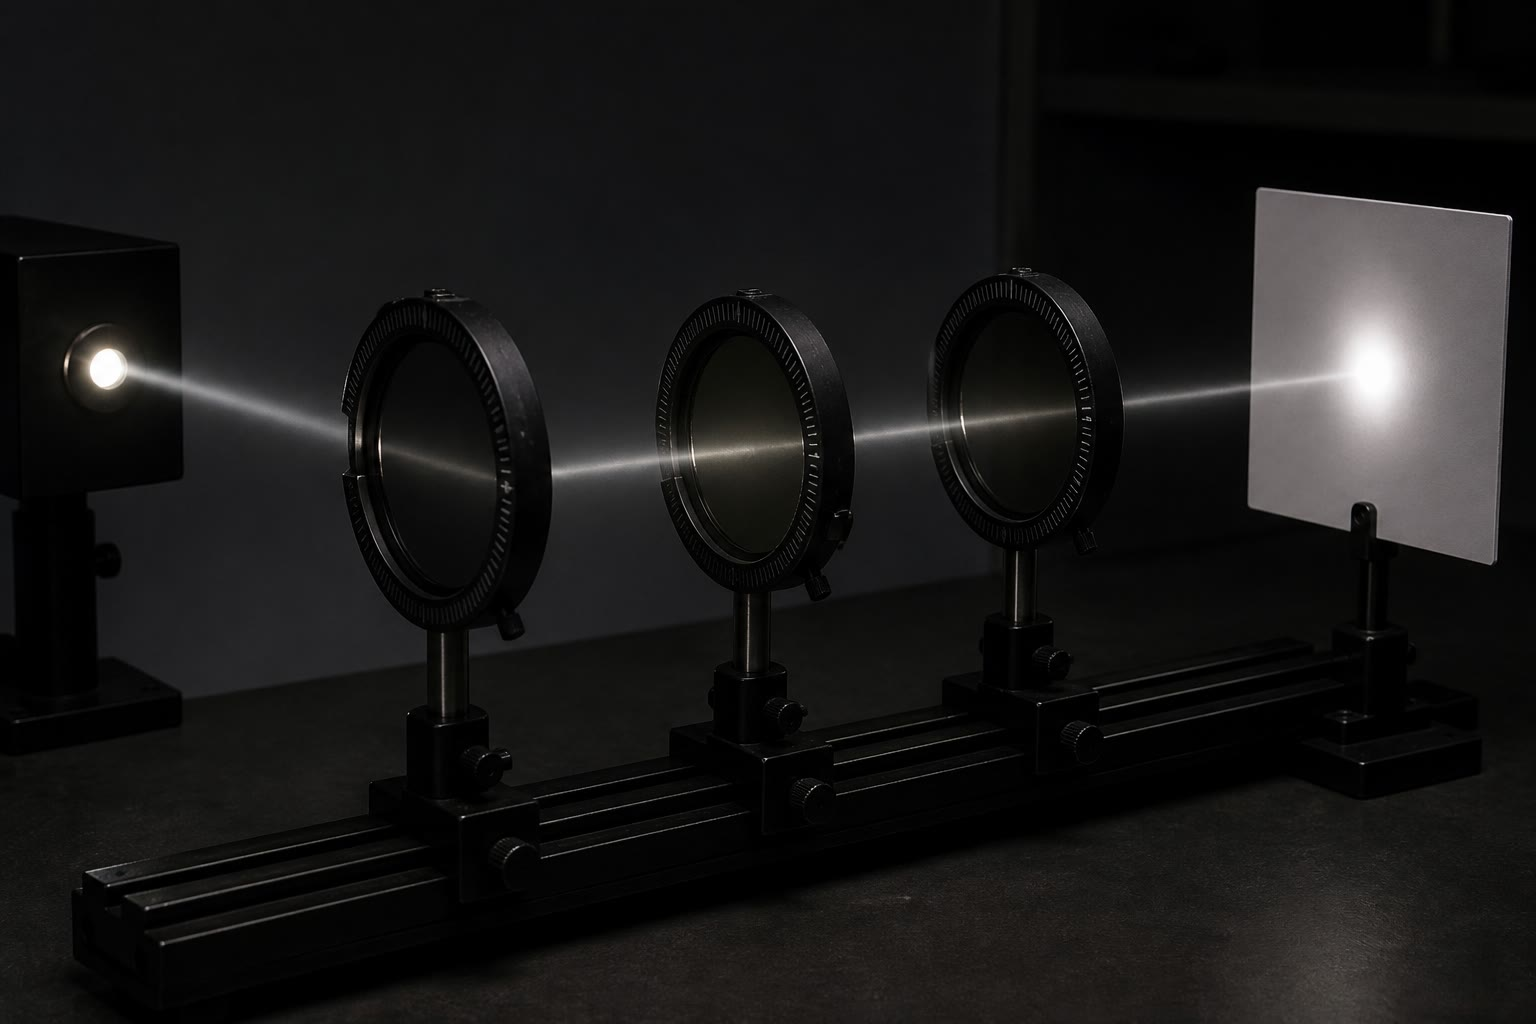
\includegraphics[width=0.58\linewidth]{images/book5/ai/b5-08-three-polarizers.jpg}

{\small 光学台上的三块起偏器：每一块都是一次测量，将光的态投影到某一轴上。两块正交放置则无光通过；在两者之间以某一角度插入第三块，光便重新透出——本章的公设，在桌面上亲手演示。}
\end{omfigure}

\section{练习}

\begin{exercise}[$\star$]\label{exo:b3:quantum-formalism:1}
在标准正交基 $(\ket1, \ket2)$ 中，设 $\ket\psi = (2\ket1 +
\iu\ket2)/\sqrt5$ 及 $\ket\varphi = (\ket1 - \ket2)/\sqrt2$。(a)
检验归一化。（b）计算 $\braket\varphi\psi$ 和
$\braket\psi\varphi$。（c）求 $\ket\psi$ 在
态 $\ket\varphi$ 中出现的概率。（d）构造与
$\ket\psi$ 正交的态（允许相差一个相位）。
\end{exercise}

\begin{exercise}[$\star$]\label{exo:b3:quantum-formalism:2}
下列哪些矩阵是厄米的，并求出这些厄米矩阵的\omterm{def:b3:quantum-formalism:observable}{本征值}
及归一化特征向量？
\[
\begin{pmatrix}0 & 1\\ 1 & 0\end{pmatrix} , \quad
\begin{pmatrix}0 & -\iu\\ \iu & 0\end{pmatrix} , \quad
\begin{pmatrix}1 & 1\\ -1 & 1\end{pmatrix} , \quad
\begin{pmatrix}2 & 1-\iu\\ 1+\iu & 3\end{pmatrix} .
\]
\end{exercise}

\begin{exercise}[$\star$]\label{exo:b3:quantum-formalism:3}
偏振角为 $\alpha$ 的光，入射到角度为
$\beta$ 的检偏器上。(a) 在 $(\ket H, \ket V)$ 基中写出两个态，并
计算透射概率。（b）导出马吕斯定律。（c）
对由 $N$ 个光子组成的光流，透射光子数的方差
是多少？（d）圆偏振光 $(\ket H + \iu\ket V)/\sqrt2$ 入射到
任意角度的线偏振检偏器上，透射概率为多少？解释
结果与角度无关的原因。
\end{exercise}

\begin{exercise}[$\star$]\label{exo:b3:quantum-formalism:4}
（a）通过作用于一个试探函数，证明 $[\hat x, \hat p] = \iu\hbar$。
（b）计算 $[\hat x^2, \hat p]$ 与 $[\hat x, \hat p^2]$。（c）证明
$[\hat A, \hat B\hat C] = [\hat A, \hat B]\hat C + \hat B[\hat A,
\hat C]$。（d）推出 $[\hat x, \hat p^n] = \iu\hbar\,n\hat p^{n-1}$，
并解释：$[\hat x, \cdot\,]$ 所模拟的是
哪一种经典运算？
\end{exercise}

\begin{exercise}[$\star\star$]\label{exo:b3:quantum-formalism:5}
连续测量。光子初始为 $\ket V$。（a）它依次经过
$45^\circ$ 与 $0^\circ$（水平）的起偏器，计算
两者都通过的概率，并明确写出中间的坍缩过程。
（b）将中间的起偏器换成两块，分别为 $30^\circ$、
$60^\circ$ 的，透射概率为多少？（c）$N - 1$ 块中间起偏器，
透振方向每次递增 $90^\circ/N$：证明生存概率为
$\cos^{2N}(\pi/2N)$，并对 $N = 2, 5, 20$ 求其值。（d）
$N \to \infty$ 的极限使偏振旋转，且\emph{无}损耗：
请评述（这一“量子芝诺”旋转已用于真实的量子比特）。
\end{exercise}

\begin{exercise}[$\star\star$]\label{exo:b3:quantum-formalism:6}
在二能级空间上，$\hat A = \begin{pmatrix}0&1\\1&0
\end{pmatrix}$, $\hat B = \begin{pmatrix}1&0\\0&-1\end{pmatrix}$.
（a）计算 $[\hat A, \hat B]$，二者是否相容？（b）态为
$\ket1$，求测量 $\hat B$ 的结果统计，再求
测量 $\hat A$ 在 $\hat B$ 测得 $+1$ \emph{之后}的结果统计。
（c）先测 $\hat A$（结果 $+1$），再测 $\hat B$，然后
再测 $\hat A$：末次 $\hat A$ 的结果与第一次的
结果\emph{相矛盾}的概率为多少？（d）若\omterm{def:b3:quantum-formalism:commutator}{对易子}为零，
这对（c）意味着什么？
\end{exercise}

\begin{exercise}[$\star\star$]\label{exo:b3:quantum-formalism:7}
（a）对
\cref{exo:b3:schrodinger-three-dimensions:1} 中的高斯态限制在一维，
计算 $\Delta x$ 与 $\Delta p$（利用傅里叶对或
直接积分），并验证海森堡关系取等号。（b）哪些态
使一般不确定性定理取等（写出
柯西–施瓦茨等号成立的条件）？（c）电子被限制在
$\Delta x = \qty{0.1}{nm}$ 内：其动能的最小量级为多少？（d）
对于局域在一微米内的弹珠（$\qty{10}{g}$），情形相同：请作出结论。
\end{exercise}

\begin{exercise}[$\star\star$]\label{exo:b3:quantum-formalism:8}
（a）由 \cref{prop:b3:quantum-formalism:evolution} 导出
$\hat x$ 与 $\hat p$ 的埃伦费斯特方程组，取 $\hat H = \hat
p^2/2m + V$。（b）证明宇称 $\hat\Pi$（$\hat\Pi\psi(x) =
\psi(-x)$）是厄米的，其平方为恒等算符，
且\omterm{def:b3:quantum-formalism:observable}{本征值}为 $\pm1$。（c）对对称势证明 $[\hat H, \hat\Pi] = 0$，
并由此推出非简并能级具有确定的宇称。
（d）对称双势阱能级的哪一个已观察到的事实，
可由此解释（回忆
本科二年级分册中的氨分子双重态）？
\end{exercise}

\begin{exercise}[$\star\star$]\label{exo:b3:quantum-formalism:9}
CSCO 的应用。在正方形二维势箱中，能级 $E
\propto 5$ 由 $\ket{1,2}$ 与 $\ket{2,1}$ 张成。（a）
证明仅凭能量不能标记态。（b）设 $\hat S$ 交换 $x
\leftrightarrow y$：证明 $\hat S$ 是厄米的，与 $\hat
H$ 对易，并求其在该能级内的本征态。（c）验证二元组 $(\hat H, \hat S)$ 能唯一标记
该能级的每一个态。（d）给出一般性的结论：
简并意味着标记集尚不完备，而
对称性提供了所缺的标记。
\end{exercise}

\begin{exercise}[$\star\star\star$]\label{exo:b3:quantum-formalism:10}
能量–时间不确定关系，严格处理。对任意\omterm{def:b3:quantum-formalism:observable}{可观测量} $\hat A$，
定义演化时间 $\tau_A = \Delta A\,/\,|\dd\langle\hat
A\rangle/\dd t|$——即均值移动一个标准
差所需的时间。（a）由 \cref{thm:b3:quantum-formalism:uncertainty} 与
\cref{prop:b3:quantum-formalism:evolution}，证明 $\Delta
E\;\tau_A \ge \hbar/2$。（b）为何这\emph{不是}
两个\omterm{def:b3:quantum-formalism:observable}{可观测量}之间的不确定关系（在该形式体系中时间是什么）？（c）应用于
一个寿命为 \qty{10}{ns} 的原子激发态：谱线宽度。（d）
应用于你的手表：一个系统的能量最多能精确到何种程度，
若其中某物每秒都有明显变化？
\end{exercise}

\begin{exercise}[$\star\star\star$]\label{exo:b3:quantum-formalism:11}
不确定性定理的证明。取 $\hat\alpha, \hat\beta$ 如
正文所设：（a）利用厄米性论证 $\Delta A^2 = \|\hat\alpha\ket\psi\|^2$，
（b）应用柯西–施瓦茨不等式，并将
$\braket{\hat\alpha\psi}{\hat\beta\psi}$ 分解为厄米部分与
反厄米部分，并将它们分别识别为反\omterm{def:b3:quantum-formalism:commutator}{对易子}与
\omterm{def:b3:quantum-formalism:commutator}{对易子}的平均值；（c）给出结论，并说明等号何时成立；
（d）证明对于 $[\hat A, \hat B] = \iu\hbar$，任何态都不能成为
两者中任一\omterm{def:b3:quantum-formalism:observable}{可观测量}的本征态，同时使两个偏差
均保持有限——并与平面波相协调。
\end{exercise}

\begin{exercise}[$\star\star\star$]\label{exo:b3:quantum-formalism:12}
看壶的水不开。二能级系统初始处于 $\ket1$，其
\omterm{def:b3:hamiltonian-mechanics:hamiltonian}{哈密顿量}驱动类拉比振荡：经过时间 $t$ 后，态为
$\cos(\omega t)\ket1 + \sin(\omega t)\ket2$（视为已知）。
（a）若不作测量，何时才完成向 $\ket2$ 的转移？
（b）在时刻 $T/N, 2T/N, \dots$ 测量“处于哪个态？”，取 $T =
\pi/2\omega$：证明在每次检测时发现系统
\emph{仍}处于 $\ket1$ 的概率为 $[\cos^2(\pi/2N)]^N$。（c）
对 $N = 1, 4, 20, 100$ 求其值，并证明它趋于 $1$：频繁
观测使演化冻结（量子芝诺效应，
1990 年用囚禁离子观测到）。（d）用一句话说明
是哪一条公设导致了这种冻结。
\end{exercise}

\begin{omfigure}
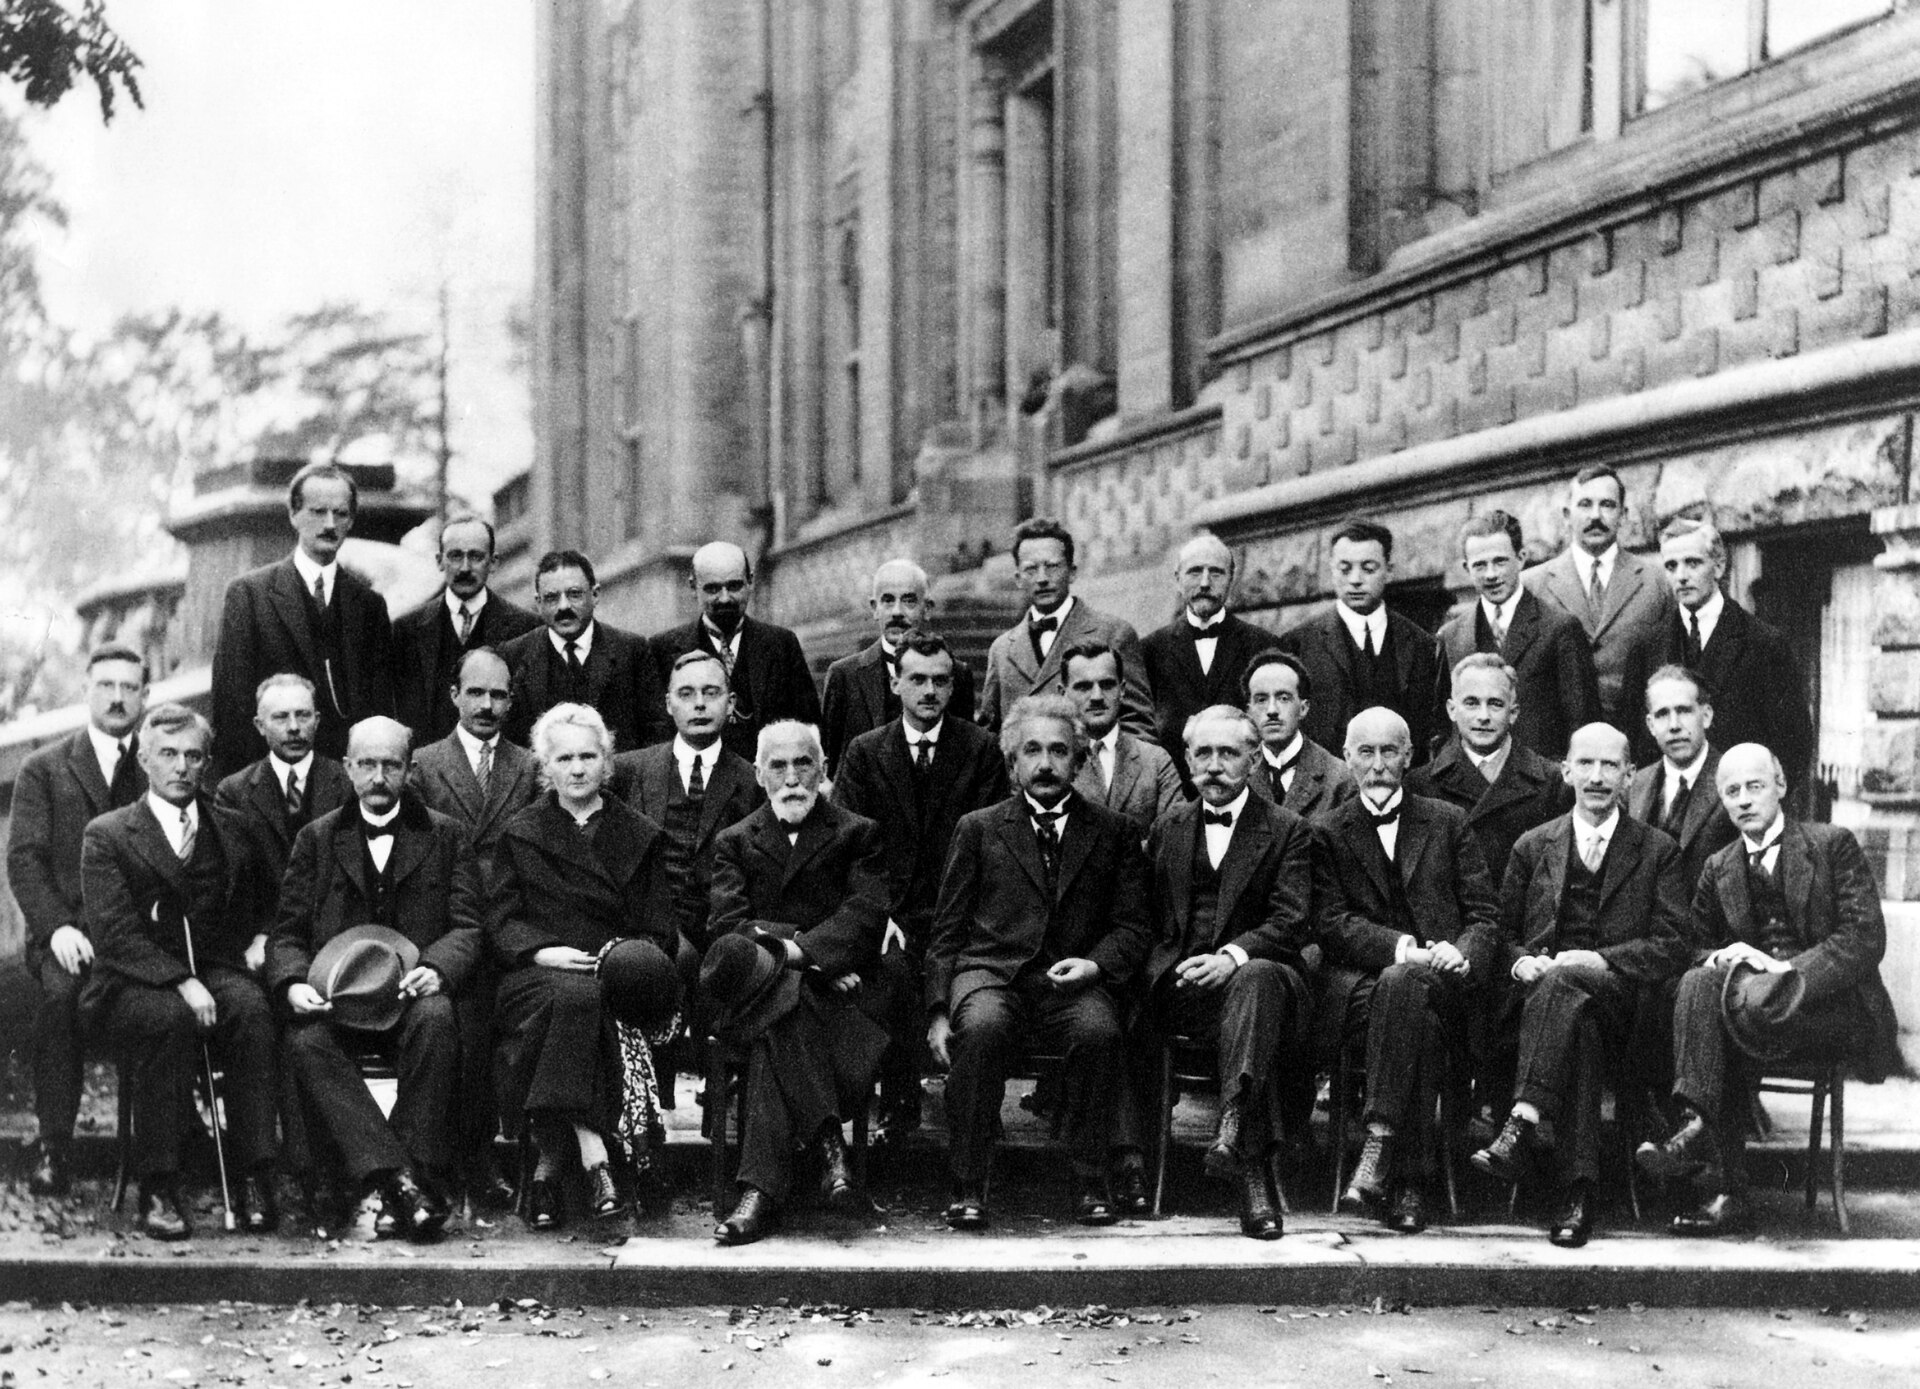
\includegraphics[width=0.62\linewidth]{images/book5/photo-solvay-1927.jpg}

{\small 1927 年索尔维会议（照片：Benjamin Couprie，公有领域）：构建本章公设的人们齐聚一室——而就在那一周，他们仍在争论测量究竟意味着什么。}
\end{omfigure}

\section{问题：中微子在飞行中更换“外衣”}

\begin{problem}[{周末问题——穿越地球的
两能级振荡}]\label{pb:b3:quantum-formalism:1}
中微子在核反应中以\emph{味}态产生——
电子中微子 $\ket{\nu_e}$ 或 μ 子中微子 $\ket{\nu_\mu}$——
但它们以能量（质量）本征态 $\ket{\nu_1},
\ket{\nu_2}$ 的形式\emph{传播}。两组基并不重合：它们之间相差一个由
\emph{混合角} $\theta$ 决定的旋转，
\[
\ket{\nu_e} = \cos\theta\,\ket{\nu_1} + \sin\theta\,\ket{\nu_2} ,
\qquad
\ket{\nu_\mu} = -\sin\theta\,\ket{\nu_1} + \cos\theta\,\ket{\nu_2} .
\]
中微子因而在飞行中\emph{振荡}于
不同味之间——从而具有质量——这一发现荣获了 2015 年
诺贝尔物理学奖。本题仅用本章的内容推导该效应，
不需超出本章的任何知识。动量为 $p$、质量为
$m_i$ 的超相对论性中微子，其能量为 $E_i \approx pc + m_i^2c^4/2pc \approx E +
m_i^2c^4/2E$。

\medskip\noindent\textbf{第一部分——形式体系的建立。}
\begin{enumerate}
  \item 验证：若 $(\ket{\nu_1}, \ket{\nu_2})$ 正交归一，则
        $(\ket{\nu_e}, \ket{\nu_\mu})$ 也正交归一。
  \item 为什么传播基必须是\emph{能量}
        本征基，而与中微子产生时所处的基无关？（哪一条
        假设支配自由传播？）
  \item 一个 μ 子中微子在 $t = 0$ 时产生，
        于质量基下写出 $\ket{\psi(0)}$。
  \item 写出 $\ket{\psi(t)}$，
        每个质量分量带有其相位 $\eu^{-\iu E_it/\hbar}$。
  \item 证明\emph{整体}相位无关紧要，并提出因子
        $\eu^{-\iu E_1t/\hbar}$：只有\emph{相对}相位
        $\Delta\phi = (E_2 - E_1)t/\hbar$ 决定物理结果。
  \item 将 $E_2 - E_1$ 用 $\Delta m^2 = m_2^2 - m_1^2$
        以及 $E$ 表示（对超相对论性中微子）。
\end{enumerate}

\medskip\noindent\textbf{第二部分——振荡公式。}
\begin{enumerate}[resume]
  \item 计算振幅 $\braket{\nu_e}{\psi(t)}$。
  \item 证明出现概率为
        \[
        \mathcal P_{\nu_\mu \to \nu_e}(t) =
        \sin^2(2\theta)\,\sin^2\Big(\frac{\Delta\phi}{2}\Big) .
        \]
        （利用 $2\sin\theta\cos\theta = \sin2\theta$。）
  \item 检验两个极限情形：$\theta = 0$ 和 $m_1 = m_2$。
        由此，任何观测到的振荡证明了什么？
  \item 取 $t \approx L/c$，证明
        \[
        \mathcal P = \sin^2(2\theta)\,
        \sin^2\Big(\frac{\Delta m^2c^4}{4\hbar c}\,\frac{L}{E}\Big) ,
        \]
        并定义振荡长度 $L_{\text{振荡}} =
        4\pi\hbar cE/\Delta m^2c^4$。
  \item 证明生存概率 $\mathcal P_{\nu_\mu \to
        \nu_\mu} = 1 - \mathcal P_{\nu_\mu\to\nu_e}$：幺正性在何处
        被用到？
  \item 为什么振荡只测量 $\Delta m^2$，
        而从不测量质量本身？
\end{enumerate}

\medskip\noindent\textbf{第三部分——解读实验。}
大气中的 μ 子中微子（$E \approx \qty{1}{GeV}$）落到探测器上，
其中从上方（$L \approx \qty{15}{km}$）与从下方来的，
后者穿过地球（$L \approx \qty{12800}{km}$）。超级神冈
（1998 年）发现，从下方来的通量减半，从上方来的通量保持不变。
\begin{enumerate}[resume]
  \item 利用 $\hbar c = \qty{197}{MeV.fm}$，证明便于使用的形式
        $\dfrac{\Delta m^2c^4\,L}{4\hbar cE} = 1.27\,
        \dfrac{\Delta m^2c^4\,[\unit{eV^2}]\ L\,[\unit{km}]}
        {E\,[\unit{GeV}]}$.
  \item 若要使振荡在 $L =
        \qty{12800}{km}$ 处\emph{充分发展}，而在 \qty{15}{km} 处\emph{可忽略}，
        在 $E = \qty{1}{GeV}$ 下，粗略界定 $\Delta m^2c^4$ 的范围。
  \item 测得值为 $\Delta m^2c^4 \approx
        \qty{2.5e-3}{eV^2}$：计算在
        \qty{1}{GeV} 下的振荡长度，并与两个基线核对。
  \item 从下方的抑制接近 $1/2$，而非 $0$：
        证明对 $\sin^2$ 在许多个振荡长度（并对能量）上\emph{求平均}，
        得到 $\tfrac12\sin^22\theta$，
        并由此推出大气混合几乎
        是\emph{最大混合}（$\theta \approx 45^\circ$）。
  \item 若较轻者可忽略，则 $\Delta m^2c^4 = \qty{2.5e-3}{eV^2}$ 给出较重质量
        本身为多少？
        将其与电子质量比较：中微子的质量
        奇异地小到何种程度？
  \item 反应堆反中微子的 $E \approx \qty{4}{MeV}$。利用同样的 $1.27$ 公式，
        证明一到两千米的基线
        恰好对准 $\qty{2.5e-3}{eV^2}$ 的分裂
        （大亚湾实验），而 $L \approx \qty{180}{km}$
        （KamLAND）则对准较小的“太阳”分裂
        $\qty{7.5e-5}{eV^2}$——用数值验证两者。
\end{enumerate}

\medskip\noindent\textbf{第四部分——含义。}
\begin{enumerate}[resume]
  \item 太阳发出 $\nu_e$；数十年来探测器只计数到预测值的
        三分之一。请用一句话分别解释“太阳中微子问题”
        及其解决方案。
  \item 为什么振荡迫使人们得出中微子
        \emph{具有质量}的结论，与标准模型最初的
        记账方式相悖？
  \item 一个量子体系在
        $12800$ 千米范围内保持相位相干，这说明中微子的相互作用
        有多弱，以及探测器为何必须极其巨大？
  \item 味道是一个\omterm{def:b3:quantum-formalism:observable}{可观测量}：为什么其算符与
        自由\omterm{def:b3:hamiltonian-mechanics:hamiltonian}{哈密顿量}不对易，
        因而味道\emph{不}存在哪一守恒律
        （而能量和动量仍守恒）？
  \item 自然界有三种味道和三种质量：为什么二能级处理
        仍能如此好地描述每个实验？
        （考虑两个 $\Delta m^2$ 的层级，
        以及每个基线分辨的是哪一个。）
  \item 在本章的形式体系中，准确指出哪些要素产生了振荡：
        哪一个基的失配、
        哪一个假设、哪一个相位。
  \item 概括这一命名结果：旋转角接近
        $45^\circ$ 与分裂 $\Delta m^2c^4 =
        \qty{2.5e-3}{eV^2}$ 使一束 GeV 的 μ 子中微子
        以振荡长度 $\sim\qty{1000}{km}$ 消失——二能级线性代数，
        并经穿过地球内部的观测所证实。
\end{enumerate}
\end{problem}
